% Chapter 1

\chapter{Introducción General} % Main chapter title

\label{Chapter1} % For referencing the chapter elsewhere, use \ref{Chapter1} 
\label{IntroGeneral}

%----------------------------------------------------------------------------------------

% Define some commands to keep the formatting separated from the content 
\newcommand{\keyword}[1]{\textbf{#1}}
\newcommand{\tabhead}[1]{\textbf{#1}}
\newcommand{\code}[1]{\texttt{#1}}
\newcommand{\file}[1]{\texttt{\bfseries#1}}
\newcommand{\option}[1]{\texttt{\itshape#1}}
\newcommand{\grados}{$^{\circ}$}

%----------------------------------------------------------------------------------------

%\section{Introducción}

%----------------------------------------------------------------------------------------
\section{Aprendiendo \LaTeX{}}

\LaTeX{} no es \textsc{WYSIWYG} (What You See is What You Get), a diferencia de los procesadores de texto como Microsoft Word o Pages de Apple. En lugar de ello, un documento escrito para \LaTeX{} es en realidad un archivo de texto simple, llano que \emph{no contiene formato} . Nosotros le decimos a \LaTeX{} cómo deseamos que se aplique el formato en el documento final escribiendo comandos simples entre el texto, por ejemplo, si quiero usar \emph{texto en cursiva para dar énfasis}, escribo \verb|\emph{texto}| y pongo el texto en cursiva que quiero entre medio de las llaves. Esto significa que \LaTeX{} es un lenguaje del tipo \enquote{mark-up}, muy parecido a HTML.

\subsection{Una introducción (no tan corta) a \LaTeX{}}

Si usted es nuevo a \LaTeX{}, hay un muy buen libro electrónico - disponible gratuitamente en Internet como un archivo PDF - llamado, \enquote{A (not so short) Introduction to \LaTeX{}}. El título del libro es generalmente acortado a simplemente \emph{lshort}. Puede descargar la versión más reciente (ya que se actualiza de vez en cuando) desde aquí:
\url{http://www.ctan.org/tex-archive/info/lshort/english/lshort.pdf}

También está disponible en varios otros idiomas. Encuentre el suyo en la lista en esta página: \url{http://www.ctan.org/tex-archive/info/lshort/}


\subsection{Guía matemática rápida para \LaTeX{}}

Si usted está escribiendo un documento con mucho contenido matemático, entonces es posible que desee leer el documento de la AMS (American Mathematical Society) llamado, \enquote{A Short Math Guide for \LaTeX{}}. Se puede encontrar en línea aquí: \url{http://www.ams.org/tex/amslatex.html} en la sección \enquote{Additional Documentation} hacia la parte inferior de la página.


%----------------------------------------------------------------------------------------

\section{Getting Started with this Template}

If you are familiar with \LaTeX{}, then you should explore the directory structure of the template and then proceed to place your own information into the \emph{THESIS INFORMATION} block of the \file{memoria.tex} file. You can then modify the rest of this file to your unique specifications based on your degree/university. Section \ref{FillingFile} on page \pageref{FillingFile} will help you do this. Make sure you also read section \ref{ThesisConventions} about thesis conventions to get the most out of this template.

If you are new to \LaTeX{} it is recommended that you carry on reading through the rest of the information in this document.

Before you begin using this template you should ensure that its style complies with the thesis style guidelines imposed by your institution. In most cases this template style and layout will be suitable. If it is not, it may only require a small change to bring the template in line with your institution's recommendations. These modifications will need to be done on the \file{MastersDoctoralThesis.cls} file.

\subsection{About this Template}

This \LaTeX{} Thesis Template is originally based and created around a \LaTeX{} style file created by Steve R.\ Gunn from the University of Southampton (UK), department of Electronics and Computer Science. You can find his original thesis style file at his site, here:
\url{http://www.ecs.soton.ac.uk/~srg/softwaretools/document/templates/}

Steve's \file{ecsthesis.cls} was then taken by Sunil Patel who modified it by creating a skeleton framework and folder structure to place the thesis files in. The resulting template can be found on Sunil's site here:
\url{http://www.sunilpatel.co.uk/thesis-template}

Sunil's template was made available through \url{http://www.LaTeXTemplates.com} where it was modified many times based on user requests and questions. Version 2.0 and onwards of this template represents a major modification to Sunil's template and is, in fact, hardly recognisable. The work to make version 2.0 possible was carried out by \href{mailto:vel@latextemplates.com}{Vel} and Johannes Böttcher.

%----------------------------------------------------------------------------------------

\section{What this Template Includes}

\subsection{Folders}

This template comes as a single zip file that expands out to several files and folders. The folder names are mostly self-explanatory:

\keyword{Appendices} -- this is the folder where you put the appendices. Each appendix should go into its own separate \file{.tex} file. An example and template are included in the directory.

\keyword{Chapters} -- this is the folder where you put the thesis chapters. A thesis usually has about six chapters, though there is no hard rule on this. Each chapter should go in its own separate \file{.tex} file and they can be split as:
\begin{itemize}
\item Chapter 1: Introduction to the thesis topic
\item Chapter 2: Background information and theory
\item Chapter 3: (Laboratory) experimental setup
\item Chapter 4: Details of experiment 1
\item Chapter 5: Details of experiment 2
\item Chapter 6: Discussion of the experimental results
\item Chapter 7: Conclusion and future directions
\end{itemize}
This chapter layout is specialised for the experimental sciences.

\keyword{Figures} -- this folder contains all figures for the thesis. These are the final images that will go into the thesis document.

\subsection{Files}

Included are also several files, most of them are plain text and you can see their contents in a text editor. After initial compilation, you will see that more auxiliary files are created by \LaTeX{} or BibTeX and which you don't need to delete or worry about:

\keyword{example.bib} -- this is an important file that contains all the bibliographic information and references that you will be citing in the thesis for use with BibTeX. You can write it manually, but there are reference manager programs available that will create and manage it for you. Bibliographies in \LaTeX{} are a large subject and you may need to read about BibTeX before starting with this. Many modern reference managers will allow you to export your references in BibTeX format which greatly eases the amount of work you have to do.

\keyword{MastersDoctoralThesis.cls} -- this is an important file. It is the class file that tells \LaTeX{} how to format the thesis. 

\keyword{memoria.pdf} -- this is your beautifully typeset thesis (in the PDF file format) created by \LaTeX{}. It is supplied in the PDF with the template and after you compile the template you should get an identical version.

\keyword{memoria.tex} -- this is an important file. This is the file that you tell \LaTeX{} to compile to produce your thesis as a PDF file. It contains the framework and constructs that tell \LaTeX{} how to layout the thesis. It is heavily commented so you can read exactly what each line of code does and why it is there. After you put your own information into the \emph{THESIS INFORMATION} block -- you have now started your thesis!

Files that are \emph{not} included, but are created by \LaTeX{} as auxiliary files include:

\keyword{memoria.aux} -- this is an auxiliary file generated by \LaTeX{}, if it is deleted \LaTeX{} simply regenerates it when you run the main \file{.tex} file.

\keyword{memoria.bbl} -- this is an auxiliary file generated by BibTeX, if it is deleted, BibTeX simply regenerates it when you run the \file{memoria.aux} file. Whereas the \file{.bib} file contains all the references you have, this \file{.bbl} file contains the references you have actually cited in the thesis and is used to build the bibliography section of the thesis.

\keyword{memoria.blg} -- this is an auxiliary file generated by BibTeX, if it is deleted BibTeX simply regenerates it when you run the main \file{.aux} file.

\keyword{memoria.lof} -- this is an auxiliary file generated by \LaTeX{}, if it is deleted \LaTeX{} simply regenerates it when you run the main \file{.tex} file. It tells \LaTeX{} how to build the \emph{List of Figures} section.

\keyword{memoria.log} -- this is an auxiliary file generated by \LaTeX{}, if it is deleted \LaTeX{} simply regenerates it when you run the main \file{.tex} file. It contains messages from \LaTeX{}, if you receive errors and warnings from \LaTeX{}, they will be in this \file{.log} file.

\keyword{memoria.lot} -- this is an auxiliary file generated by \LaTeX{}, if it is deleted \LaTeX{} simply regenerates it when you run the main \file{.tex} file. It tells \LaTeX{} how to build the \emph{List of Tables} section.

\keyword{memoria.out} -- this is an auxiliary file generated by \LaTeX{}, if it is deleted \LaTeX{} simply regenerates it when you run the main \file{.tex} file.

So from this long list, only the files with the \file{.bib}, \file{.cls} and \file{.tex} extensions are the most important ones. The other auxiliary files can be ignored or deleted as \LaTeX{} and BibTeX will regenerate them.

%----------------------------------------------------------------------------------------

\section{Filling in Your Information in the \file{memoria.tex} File}\label{FillingFile}

You will need to personalise the thesis template and make it your own by filling in your own information. This is done by editing the \file{memoria.tex} file in a text editor or your favourite LaTeX environment.

Open the file and scroll down to the second large block titled \emph{THESIS INFORMATION} where you can see the entries for \emph{University Name}, \emph{Department Name}, etc \ldots

Fill out the information about yourself, your group and institution. You can also insert web links, if you do, make sure you use the full URL, including the \code{http://} for this. If you don't want these to be linked, simply remove the \verb|\href{url}{name}| and only leave the name.

When you have done this, save the file and recompile \code{memoria.tex}. All the information you filled in should now be in the PDF, complete with web links. You can now begin your thesis proper!

%----------------------------------------------------------------------------------------

\section{The \code{memoria.tex} File Explained}

The \file{memoria.tex} file contains the structure of the thesis. There are plenty of written comments that explain what pages, sections and formatting the \LaTeX{} code is creating. Each major document element is divided into commented blocks with titles in all capitals to make it obvious what the following bit of code is doing. Initially there seems to be a lot of \LaTeX{} code, but this is all formatting, and it has all been taken care of so you don't have to do it.

Begin by checking that your information on the title page is correct. For the thesis declaration, your institution may insist on something different than the text given. If this is the case, just replace what you see with what is required in the \emph{DECLARATION PAGE} block.

Then comes a page which contains a funny quote. You can put your own, or quote your favourite scientist, author, person, and so on. Make sure to put the name of the person who you took the quote from.

Following this is the abstract page which summarises your work in a condensed way and can almost be used as a standalone document to describe what you have done. The text you write will cause the heading to move up so don't worry about running out of space.

Next come the acknowledgements. On this page, write about all the people who you wish to thank (not forgetting parents, partners and your advisor/supervisor).

The contents pages, list of figures and tables are all taken care of for you and do not need to be manually created or edited. The next set of pages are more likely to be optional and can be deleted since they are for a more technical thesis: insert a list of abbreviations you have used in the thesis, then a list of the physical constants and numbers you refer to and finally, a list of mathematical symbols used in any formulae. Making the effort to fill these tables means the reader has a one-stop place to refer to instead of searching the internet and references to try and find out what you meant by certain abbreviations or symbols.

The list of symbols is split into the Roman and Greek alphabets. Whereas the abbreviations and symbols ought to be listed in alphabetical order (and this is \emph{not} done automatically for you) the list of physical constants should be grouped into similar themes.

The next page contains a one line dedication. Who will you dedicate your thesis to?

Finally, there is the block where the chapters are included. Uncomment the lines (delete the \code{\%} character) as you write the chapters. Each chapter should be written in its own file and put into the \emph{Chapters} folder and named \file{Chapter1}, \file{Chapter2}, etc\ldots Similarly for the appendices, uncomment the lines as you need them. Each appendix should go into its own file and placed in the \emph{Appendices} folder.

After the preamble, chapters and appendices finally comes the bibliography. The bibliography style (called \option{authoryear}) is used for the bibliography and is a fully featured style that will even include links to where the referenced paper can be found online. Do not underestimate how grateful your reader will be to find that a reference to a paper is just a click away. Of course, this relies on you putting the URL information into the BibTeX file in the first place.

%----------------------------------------------------------------------------------------

\section{Thesis Features and Conventions}\label{ThesisConventions}

To get the best out of this template, there are a few conventions that you may want to follow.

One of the most important (and most difficult) things to keep track of in such a long document as a thesis is consistency. Using certain conventions and ways of doing things (such as using a Todo list) makes the job easier. Of course, all of these are optional and you can adopt your own method.

\subsection{Printing Format}

This thesis template is designed for double sided printing (i.e. content on the front and back of pages) as most theses are printed and bound this way. Switching to one sided printing is as simple as uncommenting the \option{oneside} option of the \code{documentclass} command at the top of the \file{memoria.tex} file. You may then wish to adjust the margins to suit specifications from your institution.

The headers for the pages contain the page number on the outer side (so it is easy to flick through to the page you want) and the chapter name on the inner side.

The text is set to 11 point by default with single line spacing, again, you can tune the text size and spacing should you want or need to using the options at the very start of \file{memoria.tex}. The spacing can be changed similarly by replacing the \option{singlespacing} with \option{onehalfspacing} or \option{doublespacing}.


\subsection{References}

The \code{biblatex} package is used to format the bibliography and inserts references such as this one \parencite{Reference1}. The options used in the \file{memoria.tex} file mean that the in-text citations of references are formatted with the author(s) listed with the date of the publication. Multiple references are separated by semicolons (e.g. \parencite{Reference2, Reference1}) and references with more than three authors only show the first author with \emph{et al.} indicating there are more authors (e.g. \parencite{Reference3}). This is done automatically for you. To see how you use references, have a look at the \file{Chapter1.tex} source file. Many reference managers allow you to simply drag the reference into the document as you type.

Scientific references should come \emph{before} the punctuation mark if there is one (such as a comma or period). The same goes for footnotes\footnote{Such as this footnote, here down at the bottom of the page.}. You can change this but the most important thing is to keep the convention consistent throughout the thesis. Footnotes themselves should be full, descriptive sentences (beginning with a capital letter and ending with a full stop). The APA6 states: \enquote{Footnote numbers should be superscripted, [...], following any punctuation mark except a dash.} The Chicago manual of style states: \enquote{A note number should be placed at the end of a sentence or clause. The number follows any punctuation mark except the dash, which it precedes. It follows a closing parenthesis.}

The bibliography is typeset with references listed in alphabetical order by the first author's last name. This is similar to the APA referencing style. To see how \LaTeX{} typesets the bibliography, have a look at the very end of this document (or just click on the reference number links in in-text citations).


\subsection{Tables}

Tables are an important way of displaying your results, below is an example table which was generated with this code:

{\small
\begin{verbatim}
\begin{table}
\caption{The effects of treatments X and Y on the four groups studied.}
\label{tab:treatments}
\centering
\begin{tabular}{l l l}
\toprule
\tabhead{Groups} & \tabhead{Treatment X} & \tabhead{Treatment Y} \\
\midrule
1 & 0.2 & 0.8\\
2 & 0.17 & 0.7\\
3 & 0.24 & 0.75\\
4 & 0.68 & 0.3\\
\bottomrule\\
\end{tabular}
\end{table}
\end{verbatim}
}

\begin{table}
\caption{The effects of treatments X and Y on the four groups studied.}
\label{tab:treatments}
\centering
\begin{tabular}{l l l}
\toprule
\tabhead{Groups} & \tabhead{Treatment X} & \tabhead{Treatment Y} \\
\midrule
1 & 0.2 & 0.8\\
2 & 0.17 & 0.7\\
3 & 0.24 & 0.75\\
4 & 0.68 & 0.3\\
\bottomrule\\
\end{tabular}
\end{table}

You can reference tables with \verb|\ref{<label>}| where the label is defined within the table environment. See \file{Chapter1.tex} for an example of the label and citation (e.g. Table~\ref{tab:treatments}).

\subsection{Figures}

There will hopefully be many figures in your thesis (that should be placed in the \emph{Figures} folder). The way to insert figures into your thesis is to use a code template like this:
\begin{verbatim}
\begin{figure}
\centering
\includegraphics{Figures/Electron}
\decoRule
\caption[An Electron]{An electron (artist's impression).}
\label{fig:Electron}
\end{figure}
\end{verbatim}
Also look in the source file. Putting this code into the source file produces the picture of the electron that you can see in the figure below.

%\begin{figure}[h]
%\centering
%\includegraphics{Figures/Electron}
%\decoRule
%\caption[An Electron]{An electron (artist's impression).}
%\label{fig:Electron}
%\end{figure}

Sometimes figures don't always appear where you write them in the source. The placement depends on how much space there is on the page for the figure. Sometimes there is not enough room to fit a figure directly where it should go (in relation to the text) and so \LaTeX{} puts it at the top of the next page. Positioning figures is the job of \LaTeX{} and so you should only worry about making them look good!

Figures usually should have captions just in case you need to refer to them (such as in Figure~\ref{fig:Electron}). The \verb|\caption| command contains two parts, the first part, inside the square brackets is the title that will appear in the \emph{List of Figures}, and so should be short. The second part in the curly brackets should contain the longer and more descriptive caption text.

The \verb|\decoRule| command is optional and simply puts an aesthetic horizontal line below the image. If you do this for one image, do it for all of them.

\LaTeX{} is capable of using images in pdf, jpg and png format.

\subsection{Typesetting mathematics}

If your thesis is going to contain heavy mathematical content, be sure that \LaTeX{} will make it look beautiful, even though it won't be able to solve the equations for you.

The \enquote{Not So Short Introduction to \LaTeX} (available on \href{http://www.ctan.org/tex-archive/info/lshort/english/lshort.pdf}{CTAN}) should tell you everything you need to know for most cases of typesetting mathematics. If you need more information, a much more thorough mathematical guide is available from the AMS called, \enquote{A Short Math Guide to \LaTeX} and can be downloaded from:
\url{ftp://ftp.ams.org/pub/tex/doc/amsmath/short-math-guide.pdf}

There are many different \LaTeX{} symbols to remember, luckily you can find the most common symbols in \href{http://ctan.org/pkg/comprehensive}{The Comprehensive \LaTeX~Symbol List}.

You can write an equation, which is automatically given an equation number by \LaTeX{} like this:
\begin{verbatim}
\begin{equation}
E = mc^{2}
\label{eqn:Einstein}
\end{equation}
\end{verbatim}

This will produce Einstein's famous energy-matter equivalence equation:
\begin{equation}
E = mc^{2}
\label{eqn:Einstein}
\end{equation}

All equations you write (which are not in the middle of paragraph text) are automatically given equation numbers by \LaTeX{}. If you don't want a particular equation numbered, use the unnumbered form:
\begin{verbatim}
\[ a^{2}=4 \]
\end{verbatim}

%----------------------------------------------------------------------------------------

\section{Sectioning and Subsectioning}

You should break your thesis up into nice, bite-sized sections and subsections. \LaTeX{} automatically builds a table of Contents by looking at all the \verb|\chapter{}|, \verb|\section{}|  and \verb|\subsection{}| commands you write in the source.

The Table of Contents should only list the sections to three (3) levels. A \verb|chapter{}| is level zero (0). A \verb|\section{}| is level one (1) and so a \verb|\subsection{}| is level two (2). In your thesis it is likely that you will even use a \verb|subsubsection{}|, which is level three (3). The depth to which the Table of Contents is formatted is set within \file{MastersDoctoralThesis.cls}. If you need this changed, you can do it in \file{memoria.tex}.

%----------------------------------------------------------------------------------------

\section{In Closing}

You have reached the end of this mini-guide. You can now rename or overwrite this pdf file and begin writing your own \file{Chapter1.tex} and the rest of your thesis. The easy work of setting up the structure and framework has been taken care of for you. It's now your job to fill it out!

Good luck and have lots of fun!

\begin{flushright}
Guide written by ---\\
Sunil Patel: \href{http://www.sunilpatel.co.uk}{www.sunilpatel.co.uk}\\
Vel: \href{http://www.LaTeXTemplates.com}{LaTeXTemplates.com}
\end{flushright}


%\section{Motivación}
%%----------------------------------------------------------------------------------------
%En el presente trabajo se busca satisfacer una necesidad relacionada con (...) utilizando la plataforma CIAA. 
%
%El \textit{firmware} de control se implementa sobre una de las plataformas de hardware desarrollada por el Proyecto CIAA (\textit{Computadora Industrial Abierta Argentina}), específicamente la versión CIAA-NXP. 
%
%Referencia a una sección: El Proyecto CIAA se trata en la sección \ref{sec:proyecto-ciaa}.
%
%Referencia a una figura: En la figura \ref{fig:peces} se pueden ver dos peces.
%
%Referencia a tabla: En la tabla \ref{tab:peces} se listan algunas especies de peces.
%
%Referencia a capítulo: Detalles de la implementación se abordan en el capítulo \ref{Chapter3}.
%
%\begin{figure}[h]
%\centering
%\begin{subfigure}{.5\textwidth}
%%\begin{minipage}{\linewidth}
%  \centering
%  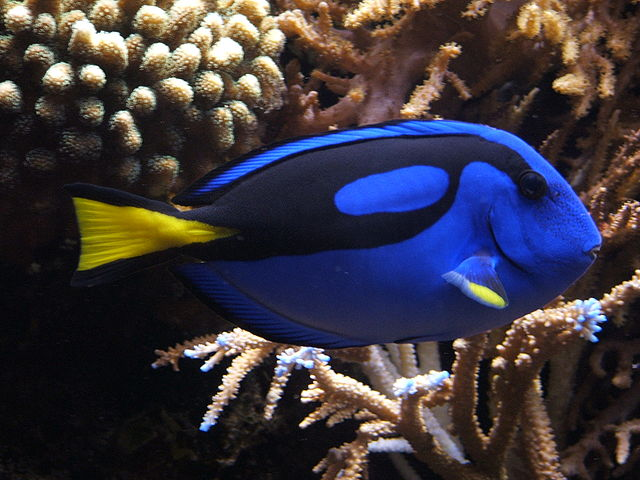
\includegraphics[height=.15\textheight]{./Figures/Dory.jpg}
%  \caption[Caption para el índice del pez 1]{pez 1\protect\footnotemark}
%  \label{fig:sub1}
%%\end{minipage}
%\end{subfigure}%
%\begin{subfigure}{.5\textwidth}
%  \centering
%  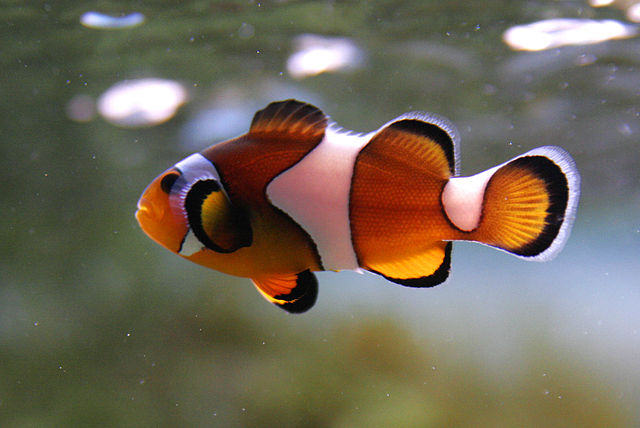
\includegraphics[height=.15\textheight]{./Figures/Nemo.jpg}
%  	\caption[caption para el pez 2]{pez 2\protect\footnotemark}
%  \label{fig:sub2}
%\end{subfigure}
%\caption{un caption para los dos peces.}
%\label{fig:peces}
%\end{figure}
%
%\footnotetext[1]{GFDL 1.2, https://commons.wikimedia.org/w/index.php?curid=654994}
%
%\footnotetext{De Tewy - Trabajo propio, CC BY 2.5, https://commons.wikimedia.org/w/index.php?curid=1382534}
%
%
%%\clearpage
%\begin{table}[ht!]
%	\centering
%	\caption[Caption de tabla para el índice.]{Costo de los peces\protect\footnotemark.}
%	\begin{tabular}{@{} l *2c @{}}    \toprule
%		\emph{\textbf{Especie}} & \emph{\textbf{Tamaño}} & \emph{\textbf{Valor aprox.}}  \\\midrule
%		Amphiprion Ocellaris			& 10 cm & \$ 6.000 \\		
%		Hepatus Blue Tang			& 15 cm	& \$	 7.000 \\
%		Zebrasoma Xanthurus			& 12 cm	& \$ 6.800 \\
%		Cirujano Naso Rubio			& 14 cm	& \$ 5.700 \\
%		Zebrasoma Cirujano			& 10 cm	& \$ 4.500 \\ 
%		Zebrasoma Desjardinii		& 10 cm 	& \$ 3.200 \\\bottomrule
%		\hline
%	\end{tabular}
%	\label{tab:peces}
%\end{table}
%
%\footnotetext{Fuente: \url{http://mercadolibre.com.ar}}
%
%Debido a la vasta difusión de las redes de computadoras y la tendencia mundial a incorporar cada día más dispositivos a Internet, fenómeno también conocido como el Internet de las cosas o \textit{Internet of Things} (IoT) se opta por desarrollar una interfaz web embebida en el dispositivo de control.  Dicha interfaz será accesible mediante el protocolo Ethernet a través de un equipo conectado a la misma red de área local o \textit{Local Area Network} (LAN).
%
%Asimismo, el control de acuarios sirve como punto de partida para desarrollar un marco de trabajo que, sin pérdida de generalidad, se puede aplicar a otros dominios de control como la domótica, agricultura inteligente, etc. En este sentido, los mecanismos utilizados en la interfaz web para comunicar al usuario con el objeto bajo control, (CGI, SSI, AJAX) no se encuentran acoplados a ninguna aplicación en particular y, dentro de un diseño modular, se pueden reutilizar en distintos proyectos.  
%
%
%\clearpage
%\section{¿Qué es un acuario?}
%\label{sec:acuario}
%
%El acuarismo es una actividad comercial y recreativa ampliamente difundida en la Argentina que consiste en establecer y mantener un ecosistema acuático artificial. El término acuario o pecera se utiliza indistintamente para referirse tanto al contenedor de agua como a todo el ecosistema artificial. 
%
%Un acuario puede albergar a un número determinado de peces, plantas e invertebrados y para su mantenimiento es preciso recrear un biotopo\footnote{Territorio o espacio vital cuyas condiciones ambientales son las adecuadas para que en él se desarrolle una determinada comunidad de seres vivos.} en función de los hábitos y costumbres de las especies que lo habiten. Existen vertebrados acuáticos aptos para vivir en agua fría, otros requieren un sistema calefactor para mantener el agua en un microclima cálido; incluso las especies marinas precisan cuidados más específicos en cuanto al tratamiento del agua.  En la figura \ref{fig:acuario} se puede observar un acuario de agua dulce sencillo, habitado por peces y plantas.
%%
%\begin{figure}[h!]
%	\centering
%    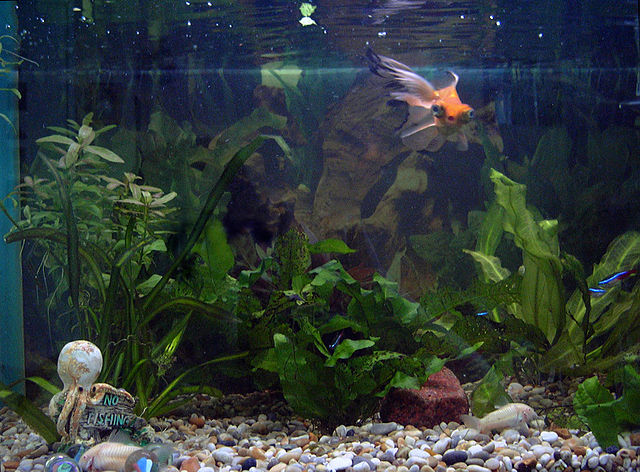
\includegraphics[width=.5\textwidth]{./Figures/acuario}
%	\caption[Acuario de agua dulce.]{Acuario de agua dulce\protect\footnotemark.}
%	\label{fig:acuario}
%\end{figure}
%
%\footnotetext{Dominio público, https://commons.wikimedia.org/w/index.php?curid=113425}
%
%Los acuarios se clasifican principalmente según las condiciones del agua:
%\begin{itemize}
%	\item Por temperatura
%	\begin{itemize}
%		\item Agua fría; entorno a los 18 \grados C.
%		\item Agua tropical; normalmente entre 22 y 27 \grados C.
%	\end{itemize}
%	\vspace{5px}
%	\item Por salinidad
%	\begin{itemize}
%		\item Agua dulce; baja concentración de sales disueltas.
%		\item Salobre; agua con entre 0.5 y 30 gr. de sal por litro.
%		\item Agua de mar o marinos; 35 gr. de sal por litro. 
%	\end{itemize}
%\end{itemize}
%
%El punto de entrada recomendado para principiantes en la disciplina es el acuario de agua dulce y fría de al menos 90 litros.  Su mantenimiento es más sencillo que el de los acuarios marinos y los peces de agua fría son los más resistentes y los que presentan mayor compatibilidad entre especies. Normalmente se pueden mantener con agua de red debidamente declorada y acondicionada. Finalmente, un acuario de mayor tamaño es más fácil de mantener, sobre todo en lo referido al tratamiento del agua y a conseguir una temperatura estable para los peces \citep{paradais1}.
%
%\subsection{Parámetros del agua}
%
%A través del agua los peces, plantas y microorganismos que habitan el acuario incorporan nutrientes y eliminan desechos. Entre ellos se conforma una cadena biológica con interacciones complejas \citep{teton2003}. A modo de ejemplo se puede mencionar cómo las colonias de microorganismos (básicamente bacterias), en etapas diferenciadas, pueden ``procesar'' los compuestos orgánicos contaminantes provenientes de los peces y plantas, y transformarlos en compuestos inofensivos o que puedan ser integrados en los tejidos de algas y plantas del acuario. En un acuario maduro se establecen ciclos beneficiosos donde lo que para unos son desechos,para otros son nutrientes.
%
%Es necesario que el agua se encuentre debidamente tratada de acuerdo con las necesidades específicas que requiera la especie de peces que se pretenda albergar.  Asimismo, se debe asegurar la mayor estabilidad de las condiciones del agua posible ya que los seres vivos que en ella habitan son sensibles a las variaciones bruscas.  
%
%Se deben tener en cuenta los siguientes parámetros del agua:
%
%\begin{itemize}
%		\item La \textbf{Dureza del agua} es una medida de la cantidad de sales minerales, particularmente las sales de calcio y magnesio, que se encuentran disueltas. Estas sales pueden ser sulfatos, cloruros, carbonatos o bicarbonatos. Nótese que la suma de todos estos compuestos es lo que se denomina Dureza Total (Gh). Los carbonatos y bicarbonatos son eliminados rápidamente debido a la evaporación del agua y gracias a las plantas (consumidoras de anhídrico carbónico). Al contenido de estas sales en el agua se lo denomina Dureza Temporal (Kh) e influye directamente en el pH del acuario. 
%		\item El valor de \textbf{Concentración de anhídrido carbónico} o $CO_2$ es fundamental para que las plantas puedan crecer y desarrollarse. La cantidad recomendada oscila entre las veinte y las treinta partes por millón (ppm).
%		\item El valor de \textbf{pH} refiere a la cantidad de iones libres de hidrógeno. Refleja el carácter ácido o alcalino del medio. El pH viene establecido por dos componentes, la dureza de carbonatos y el $CO_2$. La relación entre ambos, la dureza de carbonatos como el componente alcalino y el $CO_2$ como componente ácido, es la que establece el valor del pH en un acuario. Si la relación es similar, el pH es neutro, cercano al valor 7.
%		\item La \textbf{Temperatura} determina la actividad metabólica de los organismos dentro del acuario. Cada especie tiene un rango de temperaturas en las que puede desarrollarse con normalidad.
%\end{itemize}
%
%En general los peces viven adecuadamente en un medio con un pH que oscile entre 5 y 9. Con valores de pH extremos, tanto hacia lo ácido como hacia lo alcalino, se establecen medios sólo aptos para peces muy especiales. Normalmente, el pH más correcto para el pleno desarrollo de los peces es el que se encuentra entre 5.5 y 7.5. 
%
%
%\section{¿Qué es el Proyecto CIAA?}
%\label{sec:proyecto-ciaa}
%
%El Proyecto CIAA (Computadora Industrial Abierta Argentina) nació en 2013 como una iniciativa conjunta del sector académico y el industrial, representados por la ACSE\footnote{Asociación Civil para la investigación, promoción y desarrollo de los Sistemas electrónicos Embebidos.} y CADIEEL\footnote{Cámara Argentina de Industrias Electrónicas, Electromecánicas y Luminotécnicas.}, respectivamente \citep{CIAA}.
%
%Objetivos del proyecto:
%
%\begin{itemize}
%	\item Impulsar el desarrollo tecnológico nacional, a partir de sumar valor agregado al trabajo y a los productos y servicios, mediante el uso de sistemas electrónicos, en el marco de la vinculación de las instituciones educativas y el sistema científico-tecnológico con la industria.
%	\item Darle visibilidad positiva a la electrónica argentina.
%	\item Generar cambios estructurales en la forma en la que se desarrollan y utilizan en nuestro país los conocimientos en el ámbito de la electrónica y de las instituciones y empresas que hacen uso de ella.
%\end{itemize}
%
%Este proyecto se desarrolla en el marco de un trabajo libre, colaborativo y articulado entre industria y academia. Dentro de esta iniciativa se han elaborado distintas plataformas de \textit{hardware}, un \textit{firmware} con \textit{drivers} y ejemplos de aplicación y un entorno de desarrollo basado en Eclipse.
%
%Dentro de las plataformas de \textit{hardware} se encuentran versiones basadas en distintos microcontroladores de distintos fabricantes y versiones sobre FPGA (\textit{Field Programmable Gate Array}).  También hay versiones pensadas para trabajar en ambientes industriales y versiones educativas que utilizan el mismo microcontrolador dentro de una placa de menores prestaciones y, por lo tanto, menor costo total que la versión industrial. 
%
%A continuación se listan las plataformas que se encuentran en fase de comercialización.
%
%\begin{itemize}
%\item CIAA-NXP, primera plataforma industrial desarrollada por el proyecto.  Se basa en el microcontrolador NXP LPC4337. 
%%\vspace{5px
%\item EDU-CIAA-NXP, versión de bajo costo de la CIAA-NXP pensada para la enseñanza universitaria, terciaria y secundaria. 
%\end{itemize}
%
%Asimismo, existen otras versiones en desarrollo, CIAA-FSL, EDU-CIAA-FSL, CIAA-Safety, CIAA-ACC, EDU-CIAA-XILINX, EDU-CIAA-INTEL y CIAA-PIC. Información detallada respecto a cada plataforma y su grado de avance se puede encontrar en \citep{CIAA}.
%
%%\begin{itemize}
%%\item CIAA-FSL, basada en el microcontrolador Freescale MK60FX512VLQ15.
%%%\vspace{5px}
%%\item EDU-CIAA-FSL es una versión de bajo costo de la CIAA-FSL pensada para la enseñanza universitaria, terciaria y secundaria.
%%%\vspace{5px}
%%\item CIAA-Safety, para aplicaciones que requieran de Seguridad Funcional Certificable bajo norma IEC 61508. Basada en el microcontrolador TI RM48L952.
%%%\vspace{5px}
%%\item CIAA-ACC para aplicaciones de Alto Costo Computacional. Basada en tecnología FPGA.
%%%\vspace{5px}
%%\item EDU-CIAA-XILINX es una plataforma de bajo costo para el aprendizaje de los sistemas embebidos implementados con softcores sobre FPGA.
%%%\vspace{5px}
%%\item EDU-CIAA-INTEL es una plataforma de desarrollo de bajo costo basada en el SoM Edison de Intel.
%%%\vspace{5px}
%%\item CIAA-PIC, basada en el microcontrolador Microchip PIC32MZ2048ECH144.
%%\end{itemize}
%
%Debido a que el trabajo requiere una plataforma totalmente desarrollada y capacidad de conexión Ethernet, se elige la plataforma industrial CIAA-NXP. Se detallan en la sección \ref{sec:ciaa-nxp} las principales características de esta plataforma.
%
%\clearpage
%\subsection{Plataforma CIAA-NXP}
%\label{sec:ciaa-nxp}
%
%La CIAA-NXP es la primera y única computadora del mundo que reúne dos cualidades:
%
%\begin{itemize}
%\item 
%Ser \textbf{Industrial}, ya que su diseño está preparado para las exigencias de confiabilidad, temperatura, vibraciones, ruido electromagnético, tensiones, cortocircuitos, etc., que demandan los productos y procesos industriales.
%\item 
%Ser \textbf{Abierta}, ya que toda la información sobre su diseño de \textit{hardware}, \textit{firmware}, \textit{software}, etc. está libremente disponible en Internet bajo la Licencia BSD, para que cualquiera la utilice según sus necesidades.
%\end{itemize}
%
%\begin{figure}[h!]
%	\centering
%    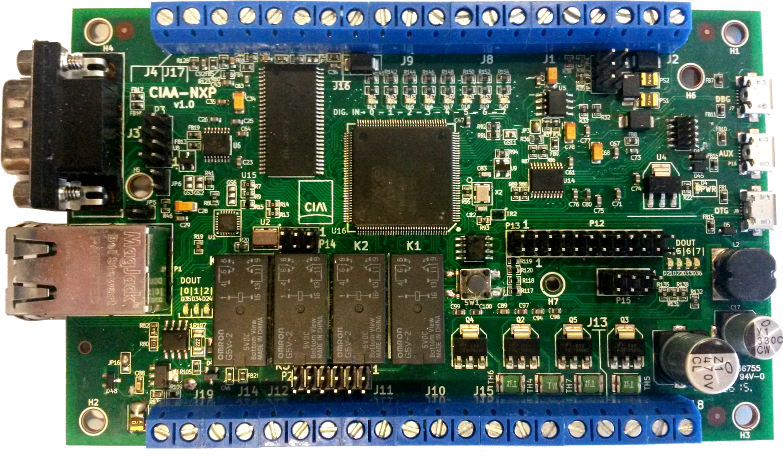
\includegraphics[width=.7\textwidth]{./Figures/ciaa-nxp.jpg}
%	\label{fig:ciaa-nxp}
%	\caption{Plataforma CIAA-NXP.}
%\end{figure}
%
%
%\noindent Esta plataforma se compone de:
%
%\begin{itemize}
%\item CPU: Microcontrolador NXP LPC4337JBD144 (Dual-core Cortex-M4 + Cortex-M0 @ 204MHz).
%\item Debugger: USB-to-JTAG FT2232H. Soportado por OpenOCD.
%\item Memorias: 
%   \begin{itemize}
%   \item IS42S16400F - SDRAM. 64Mbit @ 143MHz.
%   \item S25FL032P0XMFI011 - Flash SPI. 32 Mbit, Quad I/O Fast read: 80 MHz.
%   \item 24AA1025 - EEPROM I2C. 1 Mbit, 400 kHz. Almacenamiento de propósito general, datos de calibración del usuario, etc.
%   \item 24AA025E48 - EEPROM I2C. 2 kbit, 400 kHz. Para implementación de MAC-Address o almacenamiento de propósito general.
%   \end{itemize}
%\vspace{5px}
%\item Entradas y salidas:   
%   \begin{itemize}
%   \item 8 entradas digitales opto-acopladas.
%   \item 4 entradas analógicas 0-10V/4-20mA.
%   \item 4 salidas Open-Drain. 
%   \item 4 salidas con Relay DPDT.
%   \item 1 salida analógica 0-10V/4-20mA.
%   \end{itemize}
%\item LV-GPIO:
%   \begin{itemize}
%   \item 14 GPIOs.
%   \item I2C.
%   \item SPI.
%   \item 4 canales analógicos.
%   \item Aux. USB.
%   \end{itemize}
%\item
%Interfaces de comunicación:
%   \begin{itemize}
%   \item Ethernet.
%   \item USB On-The-Go.
%   \item RS232.
%   \item RS485.
%   \item CAN.
%   \end{itemize}
%\end{itemize}








